\documentclass[12pt,a4paper]{report}
\usepackage[utf8]{vietnam}
\usepackage[top=2cm, bottom=2cm, left=2cm, right=2cm]{geometry}
\usepackage{amsmath,amsfonts,amssymb}
\usepackage{indentfirst,enumitem}
\usepackage{graphicx}
\usepackage{multicol}
\usepackage{setspace}
\usepackage{hyperref}
\usepackage{listings}
\usepackage{tabularx}
\usepackage{hyperref}
\usepackage{xcolor}
\usepackage{scrextend}
\usepackage{comment}
\usepackage{soul}
\usepackage{tikz,tkz-tab}
%\usepackage{draftwatermark}
%\SetWatermarkText{\textsc{\LaTeX hóa bởi NhatHuy}}
%\SetWatermarkScale{0.50}
%\changefontsizes{13pt}
\renewcommand\thesection{\Roman{section}}
\renewcommand\thesubsection{\arabic{subsection}}

%New colors defined below
\definecolor{codegreen}{rgb}{0,0.6,0}
\definecolor{codegray}{rgb}{0.5,0.5,0.5}
\definecolor{codepurple}{rgb}{0.58,0,0.82}
\definecolor{backcolour}{rgb}{0.95,0.95,0.92}

%ngoặc vuông
\makeatletter
\newenvironment{sqcases}{%
  \matrix@check\sqcases\env@sqcases
}{%
  \endarray\right.%
}
\def\env@sqcases{%
  \let\@ifnextchar\new@ifnextchar
  \left\lbrack
  \def\arraystretch{1.2}%
  \array{@{}l@{\quad}l@{}}%
}
\makeatother

%Code listing style named "mystyle"
\lstdefinestyle{mystyle}{
  backgroundcolor=\color{backcolour},   commentstyle=\color{codegreen},
  keywordstyle=\color{blue},
  numberstyle=\tiny\color{codegray},
  stringstyle=\color{codepurple},
  basicstyle=\ttfamily\footnotesize,
  breakatwhitespace=false,         
  breaklines=true,                 
  captionpos=b,                    
  keepspaces=true,                 
  numbers=left,                    
  numbersep=5pt,                  
  showspaces=false,                
  showstringspaces=false,
  showtabs=false,                  
  tabsize=2
}

%"mystyle" code listing set
\lstset{style=mystyle}

\begin{document}
\begin{titlepage}
%\SetWatermarkText{\includegraphics[width = 0.97\paperwidth,
%height = 0.97\paperheight]{bia.png}}
%\SetWatermarkAngle{0} 
%\SetWatermarkText{\includegraphics[scale=1]{hust.png}}
%\SetWatermarkAngle{0} 
\begin{tikzpicture}[remember picture,overlay,inner sep=0,outer sep=0]
     \draw[blue!70!black,line width=4pt] ([xshift=-1.5cm,yshift=-2cm]current page.north east) coordinate (A)--([xshift=1.5cm,yshift=-2cm]current page.north west) coordinate(B)--([xshift=1.5cm,yshift=2cm]current page.south west) coordinate (C)--([xshift=-1.5cm,yshift=2cm]current page.south east) coordinate(D)--cycle;

     \draw ([yshift=0.5cm,xshift=-0.5cm]A)-- ([yshift=0.5cm,xshift=0.5cm]B)--
     ([yshift=-0.5cm,xshift=0.5cm]B) --([yshift=-0.5cm,xshift=-0.5cm]B)--([yshift=0.5cm,xshift=-0.5cm]C)--([yshift=0.5cm,xshift=0.5cm]C)--([yshift=-0.5cm,xshift=0.5cm]C)-- ([yshift=-0.5cm,xshift=-0.5cm]D)--([yshift=0.5cm,xshift=-0.5cm]D)--([yshift=0.5cm,xshift=0.5cm]D)--([yshift=-0.5cm,xshift=0.5cm]A)--([yshift=-0.5cm,xshift=-0.5cm]A)--([yshift=0.5cm,xshift=-0.5cm]A);


     \draw ([yshift=-0.3cm,xshift=0.3cm]A)-- ([yshift=-0.3cm,xshift=-0.3cm]B)--
     ([yshift=0.3cm,xshift=-0.3cm]B) --([yshift=0.3cm,xshift=0.3cm]B)--([yshift=-0.3cm,xshift=0.3cm]C)--([yshift=-0.3cm,xshift=-0.3cm]C)--([yshift=0.3cm,xshift=-0.3cm]C)-- ([yshift=0.3cm,xshift=0.3cm]D)--([yshift=-0.3cm,xshift=0.3cm]D)--([yshift=-0.3cm,xshift=-0.3cm]D)--([yshift=0.3cm,xshift=-0.3cm]A)--([yshift=0.3cm,xshift=0.3cm]A)--([yshift=-0.3cm,xshift=0.3cm]A);

   \end{tikzpicture}
\begin{center}
    \vspace{7pt}
    
    \textbf{ĐẠI HỌC QUỐC GIA THÀNH PHỐ HỒ CHÍ MINH}
    
    \vspace{7pt}
    \textbf{TRƯỜNG ĐẠI HỌC BÁCH KHOA}
\end{center}
\vspace{10pt}
\begin{center}
    
\includegraphics[scale=0.3]{HCMUT.png}
    
    \vspace{10pt}
    \fontsize{18pt}{17pt}\selectfont 
    \textbf{BÁO CÁO BÀI TẬP LỚN} 
    
    \vspace{7pt}
    \textbf{PHƯƠNG PHÁP TÍNH}
\end{center}

\begin{center}
    \fontsize{18pt}{17pt}\selectfont 
    \textbf{\textrm{Đề tài: Đạo hàm số trong dữ liệu tài chính}}
\end{center}

\begin{center}
    \vspace{15pt}
\textbf{Lớp: L08}
\end{center}

\begin{center}
    \vspace{15pt}
\textbf{GVHD: Võ Trần An}
\end{center}

\begin{center}
\vspace{15pt}
\textbf{Nhóm 7}
\end{center}

\vspace{10pt}

\vfill
\centerline{\bf Thành phố Hồ Chí Minh - 2024}

\vspace{1cm}
\end{titlepage}
\textbf{DANH SÁCH THÀNH VIÊN:}
\begin{table}[h]
    \begin{tabular}{|l|l|l|}
    \hline
    \textit{\textbf{Họ và tên}}   & \textit{\textbf{MSSV}} & \textit{\textbf{Phân công công việc}} \\ \hline
    \textbf{Nguyễn Đoàn Quốc Anh} & \textbf{2310093}       & \textbf{Trình bày PPT}                \\ \hline
    \textbf{Nguyễn Duy Khang}     & \textbf{2311439}       & \textbf{Chuẩn bị nội dung báo cáo}    \\ \hline
    \textbf{Nguyễn Gia Minh}      & \textbf{2312084}       & \textbf{Chuẩn bị nội dung báo cáo}    \\ \hline
    \textbf{Nguyễn Hoàng Quân}    & \textbf{2212798}       & \textbf{Chuẩn bị nội dung báo cáo}    \\ \hline
    \textbf{Nguyễn Duy Anh}       & \textbf{2310091}       & \textbf{Chuẩn bị nội dung báo cáo}    \\ \hline
    \textbf{Nguyễn Đức Thịnh}     & \textbf{2313283}       & \textbf{Thuyết trình}                 \\ \hline
    \textbf{Nguyễn Doãn Gia Huy}  & \textbf{2311173}       & \textbf{Chuẩn bị nội dung báo cáo}    \\ \hline
    \textbf{Nguyễn Bá Thành Trung}  & \textbf{2313670}       & \textbf{Chuẩn bị nội dung báo cáo}    \\ \hline
    \end{tabular}
\end{table}
\newpage    
\onehalfspacing
\tableofcontents
\newpage
\begin{center}
    \LARGE A. Giới thiệu
\end{center}
\section{Giới thiệu đề tài và mục đích nghiên cứu}
\subsection{Đề tài nghiên cứu.}
Đạo hàm số trong phân tích dữ liệu tài chính.
\subsection{Mục đích nghiên cứu.}
Thu thập, phân tích dữ liệu tài chính, dùng đạo hàm số để phân tích lợi nhuận tài chính và các yếu tố khác liên quan đến tài chính.
\section{Định nghĩa và vai trò của đạo hàm trong phân tích dữ liệu tài chính}
\subsection{Định nghĩa.}
Đạo hàm của một hàm số là một khái niệm toán học, chỉ sự biến thiên của hàm số đó khi đối số của nó thay đổi. Đạo hàm của một hàm số $f(x)$ thường được ký hiệu là $f'(x)$ hoặc là một hàm số mới mô tả tỉ lệ tăng hoặc giảm của $f(x)$ đối với đối số $x$. Nói cách khác, đạo hàm tại một điểm $x$ cho biết độ dốc của đường cong của hàm số tại điểm đó.
\subsection{Vai trò.}
Trong phân tích dữ liệu tài chính, đạo hàm có một vai trò quan trọng trong việc hiểu sự
biến động của các biến số tài chính và dự báo xu hướng của chúng. Dưới đây là một số
vai trò cơ bản của đạo hàm trong phân tích dữ liệu tài chính:
\begin{enumerate}
    \item Đánh giá Tốc độ Biến động: Đạo hàm của một hàm số tài chính thường được sử dụng để đo lường tốc độ biến động của một biến số so với thời gian. Điều này có thể giúp nhà đầu tư hoặc nhà quản lý tài chính hiểu được mức độ rủi ro hoặc cơ hội trong các khoản đầu tư hoặc quyết định kinh doanh.
    \item Xác định Điểm Cực đại và Cực tiểu: Bằng cách tìm điểm mà đạo hàm của một hàm số tài chính bằng $0$, ta có thể xác định các điểm cực đại và cực tiểu của biến số đó. Điều này giúp nhà đầu tư hoặc nhà quản lý tài chính đưa ra quyết định về thời điểm mua vào hoặc bán ra các tài sản.
    \item Dự báo Xu hướng: Bằng cách phân tích đạo hàm của một hàm số tài chính, chúng ta có thể dự báo xu hướng tương lai của biến số đó. Ví dụ, nếu đạo hàm tăng dần, có thể dự đoán rằng biến số tương ứng cũng sẽ tăng trong tương lai, và ngược lại.
    \item Xác định Tốc độ Tăng Trưởng: Đạo hàm cũng có thể giúp xác định tốc độ tăng trưởng của một biến số tài chính. Bằng cách tính đạo hàm của một hàm số tài chính tại một điểm nhất định, chúng ta có thể biết được mức độ tăng trưởng của biến số đó tại thời điểm đó.
\end{enumerate}
Tóm lại, đạo hàm đóng vai trò quan trọng trong việc phân tích dữ liệu tài chính bằng cách giúp định lượng các khía cạnh quan trọng của biến số tài chính và dự báo xu hướng tương lai.
\newpage
\begin{center}
    \LARGE B. Phương pháp nghiên cứu
\end{center}
\begin{center}
    \includegraphics*[scale = 0.2]{1.png}
\end{center}
\begin{center}
    Dữ liệu phân tích ngành trên Wichat
\end{center}
\section{Trình bày phương pháp sử dụng đạo hàm số trong phân tích dữ liệu tài chính}
Vốn dĩ toán học đã có tính ứng dụng trong kinh tế rất cao từ việc đi chợ, mua bán, tính toán chi phí… Đặc biệt, với đạo hàm thì được ứng dụng chủ yếu để biết được tốc độ tăng trưởng kinh tế nhằm đưa ra những quyết định đầu tư đúng đắn.

Đầu tiên, ta sử dụng hàm số mô tả đại lượng về kinh tế đang quan tâm, rồi tiếp đến chỉ cần áp dụng công thức tính đạo hàm để đạo hàm nó, từ đó ta sẽ dự đoán được tốc độ tăng trưởng của doanh nghiệp trong tương lai.

Ngoài ra, trong lĩnh vực kinh tế, đạo hàm còn ứng dụng tuyệt vời trong việc dự đoán xem hàm số cần tính toán đạt giá trị nhỏ nhất hay lớn nhất ở đâu, để từ đó giúp doanh nghiệp tối ưu hóa các hoạt động khác nhau một cách hiệu quả.
\begin{center}
    \includegraphics*[scale = 0.55]{2.png}
\end{center}

Dưới đây là một ví dụ về công thức tính đạo hàm lợi nhuận của một nhà sản xuất
\[
    p = \frac{-1}{3Q_3} + 14Q_2 + 60Q - 54    
\]
\newpage
Trong đó:
\begin{itemize}
    \item[-] $p$ là lợi nhuận của nhà sản xuất
    \item[-] $Q$ là mức sản lượng cho lợi nhuận $p$.
\end{itemize}
\subsubsection{Các phương pháp sử dụng đạo hàm trong phân tích dữ liệu tài chính:}
\textbf{1. Đạo hàm và xu hướng biến thiên của hàm số}

Ở dạng toán đạo hàm trong kinh tế này sẽ phải giải quyết 2 vấn đề là sự liên hệ giữa đạo hàm và xu hướng biến thiên của hàm số, cùng với việc xác định được khoảng tăng giảm của hàm số. cụ thể:
\begin{center}
    \includegraphics*[scale = 0.8]{4.png}
\end{center}

\textit{\textbf{Định lý 1: Điều kiện cần}}. Nếu hàm số $f(x)$ có đạo hàm tại mọi điểm thuộc khoảng $(a;b)$ thì:
\begin{itemize}
    \item $f(x)$ đơn điệu tăng trên khoảng $(a;b) \Rightarrow f'(x) \geq 0, \forall x \in (a;b)$.
    \item $f(x)$ đơn điệu giảm trên khoảng $(a;b) \Rightarrow f'(x) \leq 0, \forall x \in (a;b)$.
\end{itemize}

\textit{\textbf{Định lý 2: Điều kiện đủ}}. Nếu hàm số $f(x)$ có đạo hàm tại mọi điểm thuộc khoảng $(a;b)$ thì:
\begin{itemize}
    \item $f'(x) > 0, \forall x \in (a;b) \Rightarrow f(x)$ đơn điệu tăng trên khoảng $(a;b)$.
    \item $f'(x) < 0, \forall x \in (a;b) \Rightarrow f(x)$ đơn điệu giảm trên khoảng $(a;b)$.
    \item $f'(x) = 0, \forall x \in (a;b) \Rightarrow f(x)$ có giá trị không đổi trên khoảng $(a;b)$.
\end{itemize}

Xác định khoảng tăng giảm của một hàm số.

Để có thể tính toán được khoảng tăng và giảm của mộ hàm số $y = f(x)$ trong kinh tế, mọi người dựa vào những bước sau:
\begin{itemize}
    \item \textbf{Bước 1}: Xác định được miền xác định của một hàm số
    \item \textbf{Bước 2}: Tính đạo hàm $y'$ tương ứng của hàm số
    \item \textbf{Bước 3}: Tiến hành xét dấu của đạo hàm vừa tính được.
    \item \textbf{Bước 4}: Từ bảng xét dấu đạo hàm, tiến hành đưa ra kết luận khoảng tăng hay giảm của hàm số tương ứng.
\end{itemize}

\textbf{2. Tìm các điểm cực trị của hàm số}\\
Định nghĩa: Cho hàm số $f(x)$ xác định liên tục trên khoảng $(a;b)$. Trong đó:
\begin{itemize}
    \item $f(x)$ được gọi là đạt cực đại tại điểm $x_0 \in (a;b)$ nếu $\exists \delta > 0$ sao cho: $\forall x \in (a;b), 0 < | x - x_0| >< |x - x_0| < \delta \Rightarrow f(x) < f(x_0)$.
    \item $f(x)$ được gọi là đạt cực tiểu tại điểm $x_0 \in (a;b)$ nếu $\exists \delta > 0$ sao cho: $\forall x \in (a;b), 0 < | x - x_0| >< |x - x_0| < \delta \Rightarrow f(x) > f(x_0)$.
\end{itemize}
Trong đó, điểm cực tiểu và cực đại sẽ được gọi chung là điểm cực trị của một hàm số.
\begin{center}
    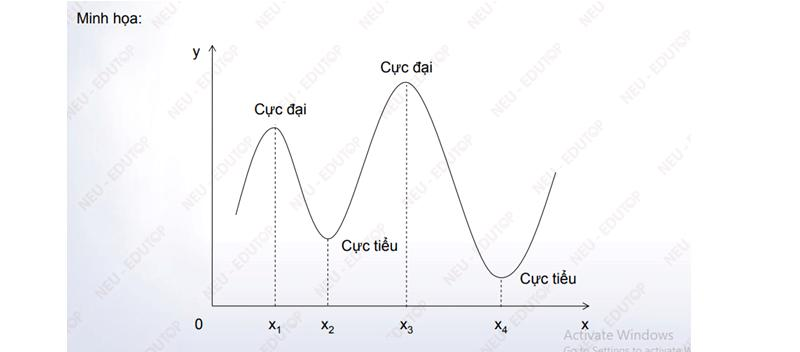
\includegraphics[scale = 0.65]{3.png}
\end{center}

Vậy nên, để có thể tìm được điểm cực trị của hàm số trong bài tập ứng dụng đạo hàm trong kinh tế, đòi hỏi phải nắm được điều kiện cần và điều kiện đủ của chúng. Cụ thể:

\textbf{Điều kiện cần:} Nếu hàm số $f(x)$ đạt cực trị tại $x_0 \in (a;b)$ và f(x) có đạo hàm tại $x_0$ thì: $f'(x0) = 0$

\textbf{Điều kiện đủ:} Giả sử $x_0$ là một trong những điểm tới hạn của một hàm số và đạo hàm của chúng có dấu xác định trên khoảng $(x_0 - d; x_0), (x_0; x_0 + d)$ của $x_0$. Nếu chúng đi qua điểm $x_0$ với đạo hàm tương ứng đổi dấu thì hàm số đó sẽ đạt cực trị tại chính điểm đó:
\begin{itemize}
    \item $x_0$ là điểm cực đại nếu $f'(x)$ đổi dấu từ + sang -.
    \item $x_0$ là điểm cực tiểu nếu $f'(x)$ đổi dấu từ - sang +.
\end{itemize}

Nếu qua điểm $x_0$ mà đạo hàm không đổi dấu thì hàm số sẽ không đạt cực trị tại điểm đó.

\textbf{Kết luận}: Hàm số $f(x)$ đưa ra chỉ có thể đạt được giá trị cực đại tại một điểm giới hạn tương ứng là -, chúng thuộc một trong hai loại là điểm dừng (điểm mà đạo hàm tại khoảng đó bị triệt tiêu) và điểm mà tại khoảng đó hàm số liên tục nhưng không có đạo hàm.

\textbf{Các bước tìm cực trị của một hàm số:}
\begin{itemize}
    \item Tìm miền xác định của hàm số tương ứng.
    \item Tìm đạo hàm của hàm số.
    \item Tính điều kiện cần của hàm số để tìm điểm tới hạn. Bao gồm tìm các điểm dừng hoặc chỉ ra những điểm thuộc miền xác định tại đó hàm liên tục nhưng không có đạo hàm.
    \item Xét điều kiện đủ của đạo hàm với từng điểm tới hạn và kết luận tương ứng.
\end{itemize}

\textbf{3. Đạo hàm và giá trị cận biên trong kinh tế}

Ở đây sẽ tiến hành tính đạo hàm cấp 1 và giá trị cận biên. Cụ thể, khi xét trên mô hình hàm số $y = f(X)$, trong đó $x$ và $y$ chính là những biến số kinh tế. Lúc này, giá trị $y-$ cận biên của $x$ tại $x = x0 (Mf(x_0))$ chính là giá trị mô tả sự thay đổi giá trị của chính $y$ khi $x$ biến đổi 1 đơn vị tại giá trị ban đầu $x = x_0$, tương ứng là $Mf(x_0) = f(x_0+1) - f(x_0)$. Khi liên hệ với đạo hàm ta có: $Mf(x_0) = f(x_0+1) - f(x-0) \approx f'(x_0)$.
\subsubsection{Một số mô hình hàm cận biên như:}
\begin{itemize}
    \item Hàm chi phí sản xuất: $TC = TC(Q)$
    \item Chi phí cận biên: $MC = TC'(Q)$
    \item Hàm doanh thu: $TR = TR(Q)$
    \item Doanh thu cận biên: $MR = TR'(Q)$
    \item Hàm lợi ích: $U = U(x)$
    \item Lợi ích cận biên: $MU = U'(x)$
    \item Hàm sản xuất ngắn hạn: $Q = f(L)$
    \item Giá trị sản phẩm hiện vật cận biên của lao động: $MPPL = f'(L)$
\end{itemize}
Ví dụ: Cho hàm sản xuất ngắn hạn: $Q = f(L) = 24\sqrt[3]{L}$. TÍnh $MPP_L$ tại các mức $L = 64$ và $L = 125$ và nêu ý nghĩa kết quả?
\[
    MPP_L \approx f'(L) = \frac{8}{\sqrt[3]{L^2}}    
\]
\begin{itemize}
    \item Tại mức $L = 64 \rightarrow MPP_L \approx f(64) = 0,5.$ Nếu tăng 1 đơn vị lao động thì sản lượng xấp xỉ $0,5$ đơn vị sản phẩm.
    \item Tại mức $L = 125 \rightarrow MPP_L \approx f(125) = 0,32.$ Nếu tăng 1 đơn vị lao động thì sản lượng xấp xỉ $0,32$ đơn vị sản phẩm.
\end{itemize}

\textbf{4. Tính đạo hàm cấp hai kèm theo quy luật lợi ích cận biên giảm dần}

Dựa trên mô hình hàm số $y= f(x)$, trong đó $y$ chính là biến số biểu diễn lợi ích của doanh nghiệp (ví dụ như lợi nhuận, doanh thu, thu nhập…) còn $x$ chính là biến số mô tả yếu tố mang lại giá trị $y$.

Quy luật lợi ích cận biên sẽ giảm dần nói rằng x càng lớn thì y cận biên càng nhỏ. Đồng thời điều kiện để \textbf{My giảm} $\Leftrightarrow f''(x) \leq 0$

\textbf{5. Tính hệ số co giãn của cung và cầu theo giá}

Việc tính hệ số co dãn của cầu theo giá chính là việc tính số do lượng thay đổi tính dựa trên $\%$ của lượng cầu khi giá tăng $1\%$. Ở đây, ta có hàm cầu $Q_D = D(p)$, tương ứng. $\varepsilon_D = \dfrac{D'(p). p}{D(p)}$.

Còn hệ số co giãn của cung theo giá chính là việc tính toán số đo lường thay đổi tính dựa trên $\%$ của lượng cung khi giá tăng $1\%$. Ở đây, ta có hàm cung $Q_S = S(p)$, tương ứng. $\varepsilon_S = \dfrac{S'(p).p}{S(p)}$

Ví dụ: Giả sử hàm cầu của người tiêu dùng đối với một loại sản phẩm có dạng:
\[
    Q_d = 1200 - p^2    
\]

Hãy tính $\varepsilon_D (10)$ và cho biết ý nghĩa kinh tế của kết quả đó.

\textbf{Giải.}\\
Ta có $Q' = -2p$
\[
    \varepsilon_D = Q' \times \frac{P}{Q} = \frac{-2p^2}{1200 - p^2} 
\]
\[
    \varepsilon_D (10) = \frac{-2\times 10^2}{1200 - 10^2}= \frac{-200}{1100} \approx 0,18
\]
Ý nghĩa: tại mức giả $p=10$, nếu tăng giá thêm $1\%$ thì lượng cầu của người tiêu dùng giảm xấp xỉ $0,18\%$.

\textbf{6. Sự lựa chọn tối ưu trong kinh tế}

Lựa chọn tối ưu trong kinh tế dựa vào đạo hàm sẽ tiến hành chọn mức sản lượng tối ưu cùng với việc chọn tối ưu mức sử dụng dựa trên yếu tố đầu vào. Cụ thể:

\begin{itemize}
    \item[a)] Chọn mức sản lượng tối ưu
        \begin{itemize}
            \item Tổng chi phí: $TC = TC(Q)$.
            \item Tổng doanh thu: $TR = TR(Q)$.
        \end{itemize}    
        Yêu cầu cần phải chọn mức sản lượng Q sao cho lợi nhuận tối đa?
        
        \textbf{Cách giải}

        Tìm Q sao cho $\pi = TR(Q) - TC(Q)$ đạt giá trị cực đại. Điều kiện cần chính là $\pi' = TR'(Q) - TC'(Q) = 0 \Leftrightarrow MR = MC$.

Lúc này, lợi nhuận sẽ đạt tối đa nếu doanh thu cận biên của công ty sẽ phải bằng chi phí cần biên. Tương ứng với điều kiện đủ chính là: $\pi''<0 \Leftrightarrow TR''(Q) > < 0 \Leftrightarrow TR''(Q) < TC''(Q)$.

Lưu ý: Khi thực hiện việc tính toán này, mọi người cần phải kiểm tra chính xác điều kiện đủ dựa trên dấu hiệu đạo hàm cấp 1 trên.
    \end{itemize}
Ví dụ: Xác định mức sản lượng tối ưu của nhà sản xuất, cho biết hàm doanh thu và chi phí như sau: $TR = 4000Q  -33Q^2$, $TC = 2Q^3 - 3Q^2 + 400Q + 5000$.

Hàm lợi nhuận là: 
\[
    \pi = TR - TC = -2Q^3 - 30Q^2 + 3600Q - 5000    
\]

Xét $\pi' = -6Q^2 - 60Q  + 3600$
\[
    \pi' = 0 \Leftrightarrow 
    \begin{sqcases}
        Q_1 = -30\\
        Q_2 = 20
    \end{sqcases}
\]

Bảng biến thiên
\begin{center}
    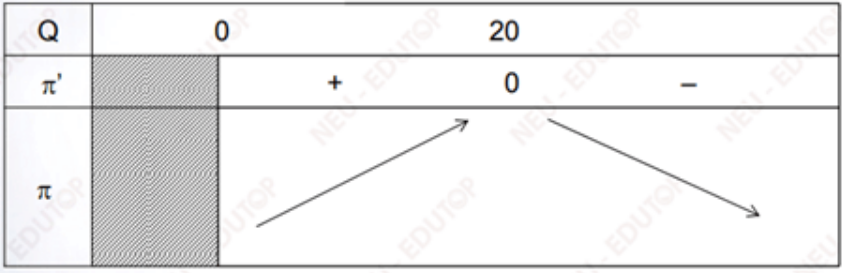
\includegraphics[scale = 0.5]{fig3.png}
\end{center}
\begin{comment}
    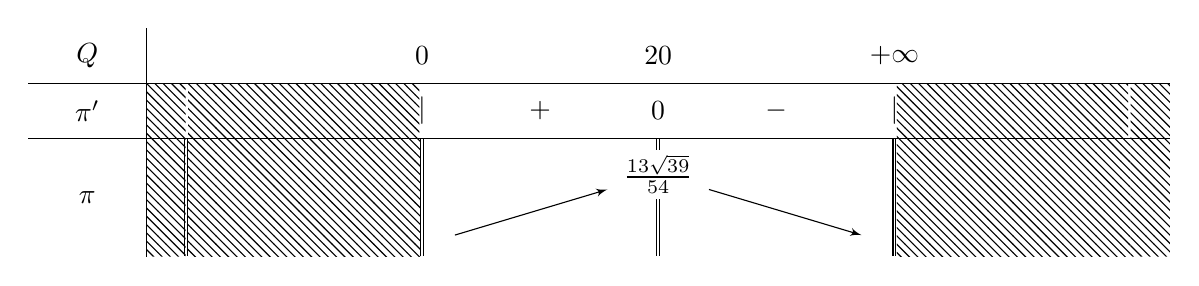
\begin{tikzpicture}
        \tikzset{h style/.style = {pattern=north west lines}} 
        \tkzTabInit[nocadre,lgt=1.5,espcl=3]
            {$Q$ /.7,$\pi'$ /.7, $\pi$ /1.5}
            {$ $,$0$,$20$,$+\infty$,$ $}
        \tkzTabLine{,h,|,+,0,-,|,h,}
        \tkzTabVar{-DH/,D-/$ $,+C/$\frac{13\sqrt{39}}{54}$,-DH/$ $}
        \pattern[pattern=north west lines] (T11)rectangle(N13)(T21)rectangle(N53);
    \end{tikzpicture}
\end{comment}

Theo bảng biến thiên, ta suy ra $\pi$ đạt giá trị lớn nhất tại $Q = 20$ $\rightarrow$ Mức sản lượng để tối ưu (sản lượng cho lợi nhuận tối đa) là $Q = 20$.
\begin{itemize}
    \item[b)] Lựa chọn tối ưu mức sử dụng dựa vào yếu tố đầu vào
    Ở đây ta sử dụng:
        \begin{itemize}
            \item Hàm sản xuất ngắn hạn tương ứng là $Q = f(L)$.
            \item Giá bán sản phẩm là $p$; giá lao động là $W_L$; chi phí cố định là $C_0$
        \end{itemize}
\end{itemize}
Lúc này hãy lựa chọn mức sử dụng lao động sao cho tiết kiệm chi phí, đạt lợi nhuận tối đa?

    \textbf{Cách giải.} Đầu tiên cần tìm $L$ sao cho $\pi = \pi.f(L) - W_L.L - C_0$ đạt được giá trị cực đại.

    Điều kiện cần tương ứng là $\pi'=0 \Leftrightarrow p.MPP_L -W_L = 0$. Lúc này, lợi nhuận sẽ đạt tối đa nếu giá trị bằng tiền của sản phẩm hiện vật cận biên của lao động sẽ bằng với giá thuê lao động.
        
    Điều kiện đủ là khi $\pi''<0 \Leftrightarrow f ''(L) >< 0 \Leftrightarrow f''(L) < 0$. Tương tự như trên thì việc điều kiện đủ có thể được xét dựa trên dấu hiệu đạo hàm cấp 1.

    Ví dụ: Một nhà sản xuất tiêu thụ sản phẩm trên thị trường cạnh tranh với giá $p = 20$USD. Cho biết hàm sản xuất $Q = 12\sqrt[3]{L^2}$ và giá thuê lao động là $W_L = 40$USD. Hãy xác định mức sử dụng lao động cho lợi nhuận tối đa.

    Hàm lợi nhuận của nhà sản xuất là:
    \[
        \pi = TR - TC = p.Q - W_L.L = 240\sqrt[3]{L^2} - 40L
    \]
    Đạo hàm:
    \[
        \pi' = \frac{160}{\sqrt[3]{L^2}} - 40
    \]
    \[
        \pi' = 0 \Leftrightarrow L = 64    
    \]

    Bảng biến thiên
    \begin{center}
        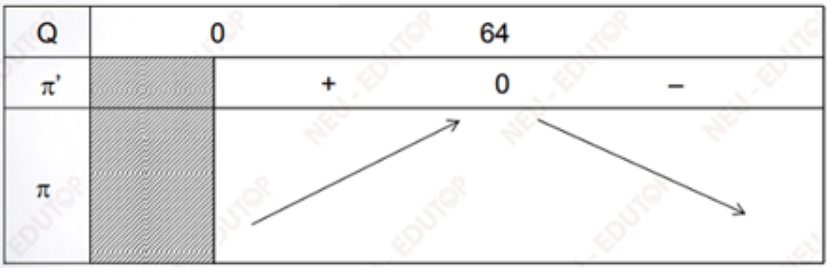
\includegraphics[scale = 0.5]{fig4.png}
    \end{center}
    Theo bảng biến thiên, ta suy ra $\pi$ đạt giá trị lớn nhất tại $L = 64$
\section{Miêu tả các công cụ phần mềm được sử dụng trong quá trình tính toán}
\textbf{MATLAB} là môi trường tính toán tương tác, cung cấp cả các chức năng cơ bản và phức tạp. Có thể sử dụng các hàm có sẵn để giải quyết các vấn đề phức tạp nhưng tiêu chuẩn hoặc bạn có thể nghĩ ra các chương trình của riêng mình bằng cách viết chúng dưới dạng tệp .m, tức là dưới dạng tệp văn bản bao gồm các dòng lệnh. Hơn nữa, MATLAB có các khả năng đồ họa phong phú mà chúng ta sẽ sử dụng với số lượng rất hạn chế, bao gồm khả năng phát triển nhanh các giao diện đồ họa người dùng.

\textbf{Một số vấn đề cơ bản có thể giải bằng Matlab:}
\begin{itemize}
    \item Giải hệ phương trình tuyến tính
    \item Giải phương trình phi tuyến theo một biến chưa biết (bao gồm phương trình đa thức là trường hợp đặc biệt).
    \item Tìm cực tiểu và cực đại của hàm một biến
    \item Hàm xấp xỉ và nội suy
    \item Tính tích phân xác định (trong không gian ít chiều)
    \item Giải phương trình vi phân thông thường, cũng như một số PDE đơn giản
\end{itemize}
\newpage
\begin{center}
    \LARGE C. Phân tích dữ liệu tài chính bằng đạo hàm số
\end{center}
\section{Phân tích lợi nhuận tài chính bằng đạo hàm số}
\begin{itemize}
    \item[-] Tính đạo hàm cột lợi nhuận theo thời gian, có thể xác định tốc độ tăng trưởng của lợi     nhuận theo từng thời điểm. Để có thể hiểu được hiệu suất kinh doanh của doanh nghiệp trong quá khứ và dự đoán xu hướng trong tương lai.
    \item[-] Các bước tính đạo hàm của cột lợi nhuận theo thời gian:
        \begin{itemize}
            \item[+]Đầu tiên, sắp xếp dữ liệu theo thời gian để có thể xác định các điểm dữ liệu liền kề theo thời gian.
            \item[+] Tiếp theo, tính toán sự thay đổi của cột lợi nhuận giữa các điểm dữ liệu liền kề. Điều này có thể được thực hiện bằng cách lấy hiệu của lợi nhuận của mỗi điểm dữ liệu so với điểm dữ liệu trước đó.
            \item[+] Sau đó, tính toán sự thay đổi của thời gian giữa các điểm dữ liệu liền kề.
            \item[+] Cuối cùng, chia sự thay đổi của lợi nhuận cho sự thay đổi của thời gian để tính toán đạo hàm của cột lợi nhuận theo thời gian.
        \end{itemize}
\end{itemize}
\textbf{Biểu diễn bằng công thức sau:}
\[
    \text{Đạo hàm lợi nhuận } = \frac{\text{lợi nhuận tại thời điểm }t_i - \text{ lợi nhuận tại thời điểm }t_{i-1}}{t_i - t_{i-1}}    
\]
Trong đó:
\begin{itemize}
    \item[+] $t_{i}$ và $t_{i-1}$ là các thời điểm liên tiếp trong dữ liệu.
    \item[+] Lợi nhuận tại thời điểm $t_{i}$ và $t_{i-1}$ là giá trị của cột lợi nhuận tại thời điểm $t_{i}$ và $t_{i-1}$.
\end{itemize}
Dùng Matlab vẽ biểu đồ lợi nhuận theo thời gian
\begin{center}
    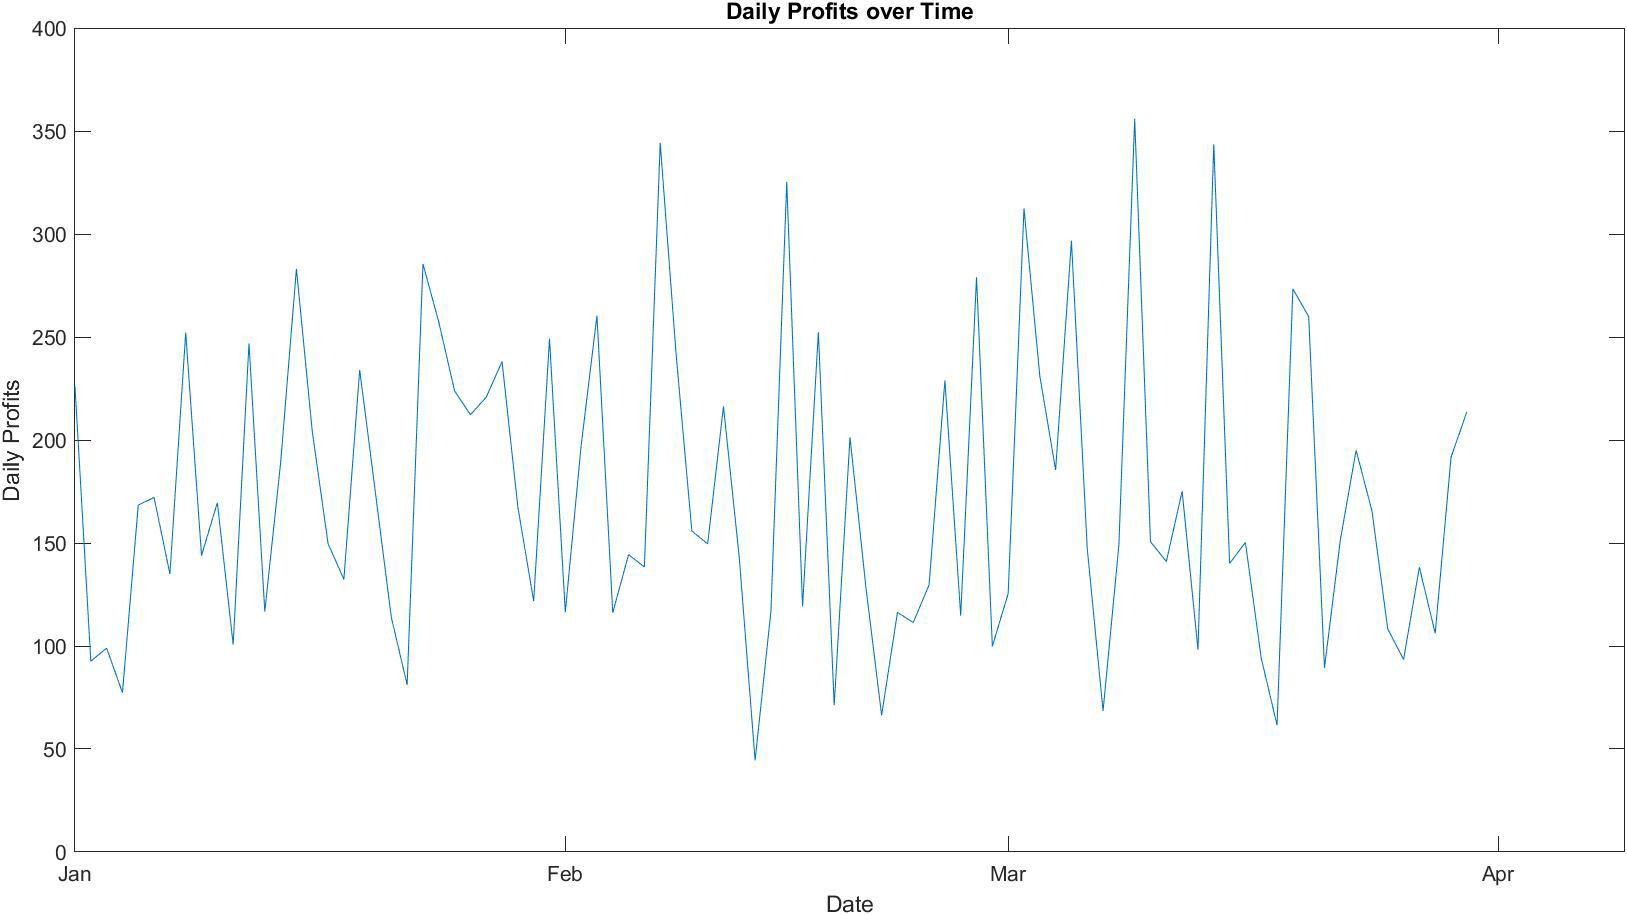
\includegraphics[scale = 0.25]{fig1.png}
\end{center}
Biểu đồ đạo hàm lợi nhuận
\begin{center}
    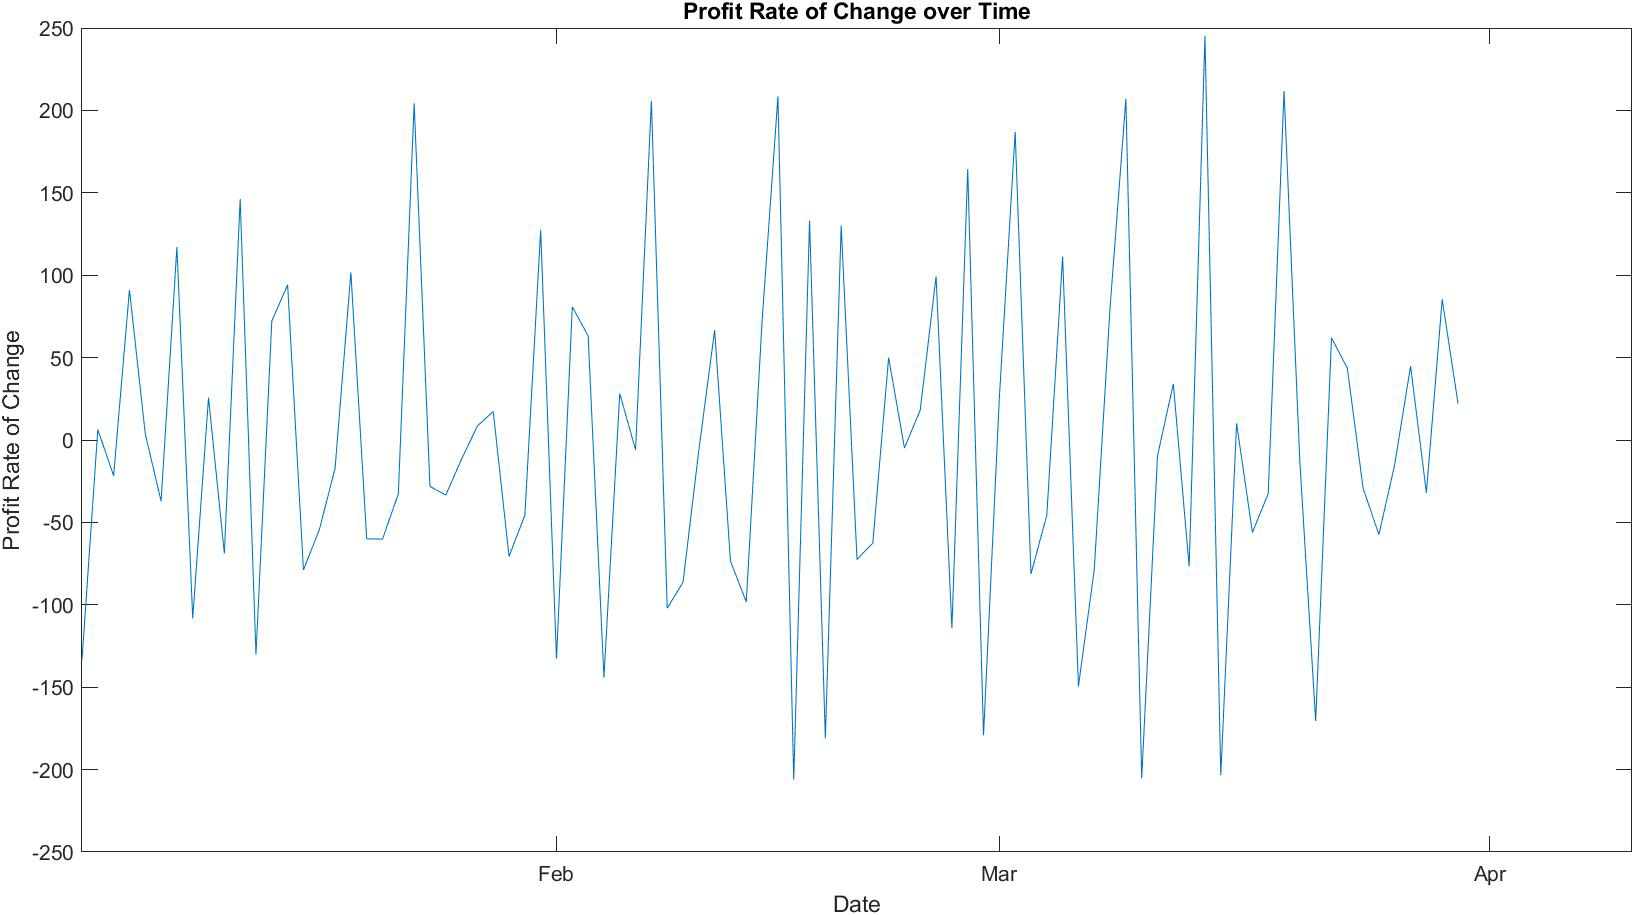
\includegraphics[scale = 0.25]{fig2.png}
\end{center}
$\rightarrow$ nhìn chung lợi nhuận ổn định, biến động lên xuống quanh 1 đường thẳng hay đạo hàm biến động quanh 0.\\
\textbf{Đoạn code Matlab}
\lstinputlisting[language=Matlab]{code.m}
\section{Phân tích các yếu tố khác liên quan đến tài chính bằng cách áp dụng đạo hàm số}
\subsection{Tốc độ tăng trưởng}
\subsubsection{* Ý nghĩa tốc độ tăng trưởng}
\textbf{Tốc độ tăng trưởng tài chính (Financial Growth Rate)}: Đạo hàm của hàm tăng trưởng tài chính theo thời gian có thể cung cấp thông tin về mức độ biến động của tốc độ tăng trưởng. Nếu tốc độ tăng trưởng giảm, điều này có thể chỉ ra sự chậm trễ trong việc phát triển kinh doanh hoặc sự suy giảm của ngành công nghiệp.
\subsubsection{* Vai trò đạo hàm số trong tốc độ tăng trưởng}
\textbf{Phân tích độ nhạy của tốc độ tăng trưởng}: Bằng cách sử dụng đạo hàm riêng, chúng ta có thể xác định độ nhạy của tốc độ tăng trưởng tài chính đối với các biến số khác nhau. Điều này giúp xác định những yếu tố nào có ảnh hưởng mạnh mẽ nhất đến tăng trưởng tài chính.

\textbf{Dự báo tốc độ tăng trưởng}: Bằng cách sử dụng phương pháp đạo hàm, chúng ta có thể tạo ra các mô hình dự báo tốc độ tăng trưởng dựa trên các yếu tố tài chính khác nhau và dự báo những thay đổi trong tương lai.

\textbf{Đánh giá rủi ro tài chính}: Bằng cách phân tích biến động của đạo hàm của tốc độ tăng trưởng, chúng ta có thể đánh giá rủi ro tài chính và xác định mức độ ảnh hưởng của các yếu tố khác nhau đối với sự ổn định tài chính.
\subsection{Điểm cực đại và cực tiểu}
\subsubsection{* Ý nghĩa điểm cực đại và cực tiểu}
\textbf{Tìm điểm cực đại và cực tiểu của hàm lợi nhuận}: Bằng cách tìm đạo hàm của hàm lợi nhuận theo các biến số tài chính như doanh thu, chi phí, hoặc giá cổ phiếu, chúng ta có thể xác định các điểm cực đại và cực tiểu của lợi nhuận. Điều này giúp chúng ta hiểu rõ hơn về cách các yếu tố tài chính ảnh hưởng đến hiệu suất kinh doanh. 
\subsubsection{* Vai trò điểm cực đại và cực tiểu}
\textbf{Đánh giá hiệu quả của chiến lược đầu tư}: Bằng cách đạo hàm số ta tìm ra cực đại của hàm lợi nhuận hoặc giảm thiểu của hàm chi phí đối với các biến số như lãi suất, thời gian đầu tư, hoặc mức độ rủi ro, chúng ta có thể đánh giá hiệu quả của các quyết định đầu tư và chiến lược tài chính.

\textbf{Xác định giá trị tối ưu của các sản phẩm hoặc dịch vụ}: Bằng cách đạo hàm số ta tìm được cực đại của hàm doanh thu hoặc lợi nhuận theo các biến số như giá cả, khuyến mãi, hoặc quảng cáo, chúng ta có thể xác định giá trị tối ưu của các sản phẩm hoặc dịch vụ.

\textbf{Quản lý rủi ro tài chính}: Bằng cách đạo hàm số ta phân tích được cực đại và cực tiểu của hàm rủi ro tài chính theo các biến số như tỷ lệ nợ vay, tỷ lệ vốn chủ sở hữu, hoặc đòn bẩy tài chính, chúng ta có thể xác định các chiến lược quản lý rủi ro tối ưu.

\textbf{Đánh giá tác động của chính sách tài chính}: Bằng cách đạo hàm số ta tìm ra cực đại hoặc cực tiểu của hàm tài chính theo các biến số như thuế suất, lãi suất, hoặc mức độ hỗ trợ từ chính phủ, chúng ta có thể đánh giá tác động của các chính sách tài chính đối với các tổ chức và thị trường.
\subsection{Biến động và ổn định của dữ liệu tài chính}
Phân tích biến động và ổn định của dữ liệu tài chính bằng đạo hàm số có thể được thực hiện bằng cách sử dụng các phương pháp thống kê và toán học để đánh giá xu hướng, biến động và sự biến đổi của các chỉ số tài chính. Điều này có thể bao gồm việc tính toán đạo hàm của các hàm số thể hiện các chỉ số tài chính để đo lường sự biến động và ổn định của chúng theo thời gian.

* Sử dụng đạo hàm số để phân tích biến động và ổn định của dữ liệu tài chính có thể bao gồm các bước như sau:\\
\textbf{a) Chọn chỉ số tài chính cần phân tích}: Chọn các chỉ số như giá cổ phiếu, lợi nhuận, doanh số bán hàng, hoặc các chỉ số tài chính khác.

Để phân tích, hãy chọn một chỉ số tài chính như giá cổ phiếu của một công ty cụ thể. Giá cổ phiếu thường được xem xét kỹ lưỡng trong phân tích tài chính vì nó phản ánh sự khả quan của thị trường đối với hiệu suất và triển vọng của công ty đó.\\
\textbf{b) Xây dựng hàm số biểu diễn dữ liệu}: Xây dựng hàm số hoặc mô hình thống kê để biểu diễn dữ liệu tài chính. Ví dụ, có thể sử dụng một phương trình để biểu diễn giá cổ phiếu theo thời gian.

Một phương trình đơn giản để biểu diễn giá cổ phiếu theo thời gian có thể là một phương trình hồi quy tuyến tính, trong đó giá cổ phiếu được ước lượng dựa trên thời gian và các biến khác có thể ảnh hưởng đến giá cổ phiếu, như chỉ số thị trường, lợi nhuận công ty, hoặc các yếu tố kinh tế khác. Ví dụ, một phương trình đơn giản có thể là:
\[
    P(t) = a.t + b
\]
\newpage
Trong đó:
\begin{itemize}
    \item[-] $P(t)$ là giá cổ phiếu tại thời điểm.
    \item[-] $a$ là hệ số của thời gian.
    \item[-] $b$ là hệ số giao cắt (giá cổ phiếu tại thời điểm ban đầu).
\end{itemize}

Để có một phân tích chính xác hơn, có thể sử dụng mô hình thống kê phức tạp hơn, chẳng hạn như mô hình quy hồi đa biến hoặc mô hình dự báo chuỗi thời gian.\\
\textbf{c) Tính đạo hàm của hàm số}: Sử dụng phép tính đạo hàm để tính toán biến đổi của hàm số theo thời gian. Điều này có thể cho thấy tốc độ thay đổi của chỉ số tài chính.

Để tính toán đạo hàm của hàm số biểu diễn giá cổ phiếu theo thời gian, chúng ta sẽ lấy đạo hàm của hàm số đó theo biến thời gian $t$ .Trong trường hợp phương trình đơn giản $P(t)= at + b$, đạo hàm của $P(t)$ theo $t$ sẽ là $a$, tức là hệ số của thời gian. Điều này cho thấy tốc độ thay đổi của giá cổ phiếu là hằng số $a$. Trong trường hợp mô hình phức tạp hơn, chẳng hạn một mô hình hồi quy đa biến, việc tính toán đạo hàm có thể phức tạp hơn và có thể đòi hỏi sử dụng các phương pháp tính toán đạo hàm riêng biệt cho mỗi biến độc lập trong mô hình.\\
\textbf{d) Phân tích biến động}: Đánh giá biến động của đạo hàm để xác định các điểm cực đại, cực tiểu hoặc điểm uốn của hàm số. Các biến động lớn có thể biểu thị sự không ổn định trong dữ liệu tài chính.

Phân tích biến động trong việc đánh giá biến động của đạo hàm là một phương pháp quan trọng để xác định các điểm cực đại, cực tiểu hoặc điểm uốn của một hàm số. Các biến động lớn thường cho thấy sự không ổn định trong dữ liệu tài chính và có thể có ảnh hưởng lớn đến quyết định đầu tư và phân tích rủi ro. Để thực hiện phân tích biến động, ta thường làm những bước sau:
\begin{enumerate}
    \item \textbf{Tìm đạo hàm}: Đầu tiên, ta tìm đạo hàm của hàm số cần phân tích. Đạo hàm thường được sử dụng để biểu diễn sự thay đổi của hàm số theo biến số.
    \item \textbf{Xác định điểm cực đại và cực tiểu}: Điểm cực đại là điểm mà đạo hàm đổi dấu từ dương sang âm, và điểm cực tiểu là điểm mà đạo hàm đổi dấu từ âm sang dương. Các điểm này thường là các điểm mà hàm số đạt giá trị lớn nhất hoặc nhỏ nhất.
    \item \textbf{Xác định điểm uốn}: Điểm uốn là điểm mà đạo hàm thay đổi hướng của độ dốc, tức là từ tăng sang giảm hoặc từ giảm sang tăng. Điểm uốn thường cho thấy sự thay đổi của tốc độ tăng trưởng của hàm số.
    \item \textbf{Đánh giá biến động}: Bằng cách quan sát sự biến động của đạo hàm xung quanh các điểm cực đại, cực tiểu và điểm uốn, chúng ta có thể đánh giá mức độ ổn định của hàm số và dữ liệu tài chính tương ứng. Trong phân tích tài chính, việc nhận biết và đánh giá biến động quan trọng để đưa ra các quyết định thông minh trong việc quản lý rủi ro và đầu tư.
\end{enumerate}
\textbf{e) Đánh giá ổn định}: Xem xét độ lớn của đạo hàm và cách nó thay đổi qua thời gian để đánh giá sự ổn định của dữ liệu tài chính. Sự dao động nhỏ có thể cho thấy sự ổn định.\\

Đánh giá ổn định của dữ liệu tài chính thông qua đạo hàm là một cách tiếp cận thông minh. Dưới đây là các bước thường được thực hiện trong quá trình này:
\begin{enumerate}
    \item \textbf{Xem xét độ lớn của đạo hàm}: Độ lớn của đạo hàm thường biểu thị tốc độ thay đổi của hàm số. Nếu đạo hàm có giá trị lớn, điều này có thể chỉ ra sự biến động mạnh mẽ trong dữ liệu tài chính.
    \item \textbf{Quan sát cách đạo hàm thay đổi qua thời gian}: Bằng cách xem xét sự biến động của đạo hàm qua các khoảng thời gian khác nhau, ta có thể đánh giá sự ổn định của dữ liệu. Nếu đạo hàm thay đổi đều đặn và không có biến động lớn, điều này có thể cho thấy sự ổn định của dữ liệu.
    \item \textbf{Xác định sự dao động nhỏ}: Sự dao động nhỏ của đạo hàm thường là dấu hiệu của sự ổn định trong dữ liệu tài chính. Nếu đạo hàm biến động nhỏ và duy trì ở mức thấp qua nhiều khoảng thời gian, điều này có thể cho thấy sự ổn định của dữ liệu.
    \item \textbf{So sánh với ngưỡng ổn định}: Đôi khi, ta cũng có thể đặt ra một ngưỡng cụ thể cho sự biến động của đạo hàm để đánh giá sự ổn định của dữ liệu. Nếu biến động của đạo hàm không vượt quá ngưỡng này, có thể kết luận rằng dữ liệu đang ổn định. Đánh giá ổn định thông qua đạo hàm cung cấp một cái nhìn đa chiều và kỹ lưỡng về sự biến động của dữ liệu tài chính, giúp nhà đầu tư và nhà quản lý rủi ro đưa ra các quyết định thông minh và có căn cứ.    
\end{enumerate}
\textbf{f) Kết luận và đề xuất}: Dựa trên phân tích, đưa ra kết luận về biến động và ổn định của dữ liệu tài chính và đề xuất các biện pháp cần thiết nếu cần.\\

Dựa trên phân tích về biến động và ổn định của dữ liệu tài chính, dưới đây là một kết luận tổng quan cùng với các đề xuất có thể được đưa ra:
\subsection*{Kết luận}
\begin{enumerate}
    \item \textbf{Biến động của dữ liệu}: Phân tích biến động của đạo hàm đã cho thấy rằng dữ liệu tài chính hiện đang trải qua một mức độ biến động đáng kể. Điều này có thể phản ánh sự không ổn định trong thị trường hoặc trong các yếu tố kinh tế liên quan.
    \item \textbf{Ổn định của dữ liệu}: Mặc dù có biến động, tuy nhiên, dữ liệu tài chính vẫn cho thấy một mức độ ổn định trong một số khía cạnh. Sự dao động của đạo hàm không vượt quá một ngưỡng nhất định và duy trì ở mức tương đối thấp trong một khoảng thời gian đáng kể.    
\end{enumerate}
\subsection*{Đề xuất}
\begin{enumerate}
    \item \textbf{Tăng cường giám sát}: Do biến động của dữ liệu, việc tăng cường giám sát và theo dõi thị trường là cần thiết. Cần thiết phải duy trì một cơ chế giám sát chặt chẽ để nắm bắt những biến động và thay đổi mới trong thị trường và dữ liệu tài chính.
    \item \textbf{Đa dạng hóa danh mục đầu tư}: Trong bối cảnh biến động, đa dạng hóa danh mục đầu tư có thể là một biện pháp phòng ngừa hiệu quả. Việc phân chia đầu tư vào nhiều tài sản khác nhau có thể giúp giảm thiểu rủi ro và bảo vệ lợi ích của nhà đầu tư.
    \item \textbf{Đánh giá lại chiến lược đầu tư}: Nếu biến động của dữ liệu tài chính gây ra sự không ổn định đáng kể trong chiến lược đầu tư, cần xem xét và đánh giá lại chiến lược đó để đảm bảo rằng nó vẫn phù hợp với tình hình thị trường hiện tại.
    \item \textbf{Đào tạo và chuẩn bị cho nhân viên}: Đảm bảo rằng nhân viên liên quan đến quản lý rủi ro và đầu tư được đào tạo đầy đủ và có kiến thức vững về cách xử lý và phản ứng với biến động trong dữ liệu tài chính.
    \item \textbf{Nâng cao khả năng dự đoán}: Sử dụng công nghệ và các công cụ phân tích dữ liệu tiên tiến để nâng cao khả năng dự đoán và đưa ra quyết định dựa trên thông tin chính xác và chi tiết. Bằng cách thực hiện các biện pháp này, ta có thể làm giảm thiểu rủi ro và tối ưu hóa hiệu suất trong môi trường tài chính đang biến động.    
\end{enumerate}
\section{Kết quả và thảo luận}
Phân tích dữ liệu tài chính bằng đạo hàm số thường được sử dụng để đo lường sự biến động của dữ liệu, như tỉ lệ tăng trưởng, biến động trong thời gian, và tốc độ thay đổi của các chỉ số tài chính. Điều này giúp nhà đầu tư và nhà quản lý tài chính hiểu rõ hơn về xu hướng và rủi ro trong thị trường tài chính.
\newpage
\section{Tài liệu tham khảo}
\begin{itemize}
    \item[$\lbrack1\rbrack$] Brandimarte. (2006). \textit{Numerical methods in finance and economics: A MATLAB-based introduction}. John Wiley $\&$ Sons.
    \item[$\lbrack2\rbrack$] Lê Thái Thanh (2017). \textit{Giáo trình Phương pháp tính}, Nhà xuất bản Đại học quốc gia TP Hồ Chí Minh.
    \item[$\lbrack3\rbrack$] Quang N. H. (2023, September 13). Dữ liệu tài chính là gì? Tại sao cần sử dụng dữ liệu tài chính trong đầu tư. WiGroup. https://www.wigroup.vn/post/du-lieu-tai-chinh-la-gi-tai-sao-can-su-dung-trong-dau-tu-wichart
\end{itemize}
\end{document}